% !TEX root = index.tex

%basic AMS packages
\documentclass[reqno,letter, 11pt,twoside]{article}
\usepackage{amsmath}
\usepackage{amsthm}
\usepackage{amssymb}
\usepackage{hyperref}
\hypersetup{
	colorlinks = true,
	linkcolor = blue,
	anchorcolor = blue,
	citecolor = blue,
	filecolor = blue,
	urlcolor = blue
}
\usepackage{epigraph}
\usepackage{mathpazo}
\usepackage{tcolorbox}
\usepackage[margin=1in,includehead,includefoot]{geometry}
\usepackage{fancyhdr}
  \pagestyle{fancy}
  \fancyhf{}
  \fancyhead[LO]{Cohomology via Sheaves}
  \fancyhead[RE]{Apurva}
  \fancyhead[LE]{Mathcamp}
  \cfoot{\thepage}

\usepackage{graphicx}
  \graphicspath{ {images/} }
\usepackage{float}
\usepackage{subcaption}
\usepackage{color}
\usepackage{mdframed}
\usepackage{enumitem}
  \setlist[enumerate]{label=\emph{\alph*})}% global settings, for all lists
\usepackage{tikz}
\usepackage[all,cmtip]{xy}
\usepackage{multicol}
% \renewcommand{\thefootnote}{\fnsymbol{footnote}}

% \makeatletter
% \@addtoreset{footnote}{section}
% \makeatother

%for setting the equation number to sync with the theorem numbers
\numberwithin{equation}{section}
\newcommand{\hint}[1]{\footnote{\raggedleft\rotatebox{180}{Hint: #1\hfill}}}

%How does latex not have these?
\DeclareMathOperator{\Ad}{Ad}
\DeclareMathOperator{\ad}{ad}
\DeclareMathOperator{\tr}{tr}
\DeclareMathOperator{\Tr}{Tr}
\DeclareMathOperator{\Hom}{Hom}
\DeclareMathOperator{\maps}{Maps}
\DeclareMathOperator{\im}{im}
\DeclareMathOperator{\rank}{rank}
\DeclareMathOperator{\coker}{coker}
\DeclareMathOperator{\Exists}{\exists}
\DeclareMathOperator{\Forall}{\forall}
\DeclareMathOperator{\res}{Res}
\DeclareMathOperator{\mor}{Res}

%simple operators which can be pretty useful
\newcommand{\pr}[2][\:]{\frac{\partial #1}{\partial #2}}
\newcommand{\innerp}[2]{\langle #1, #2 \rangle}
\newcommand*\conj[1]{\overline{#1}}
\newcommand*\norm[1]{\lVert #1 \rVert}

\theoremstyle{plain}
\newtheorem{thm}{Theorem}[section]
\newtheorem{prop}[thm]{Proposition}
\newtheorem{lem}[thm]{Lemma}
\newtheorem{cor}[thm]{Corollary}


\theoremstyle{definition}
\newtheorem{definition}[thm]{Definition}
\newtheorem{example}[thm]{Example}
\newtheorem{remark}[thm]{Remark}
\newtheorem{ans}[thm]{Ans.}

\newcounter{q}
\newtheorem{question}[q]{Question.}
\definecolor{light-gray}{gray}{0.95}
\newenvironment{ques}
{
	\begin{tcolorbox}[colback=light-gray,arc=0pt,outer arc=0pt,boxrule=0.5pt]
	 \begin{question}
			}
			{
		\end{question}
	\end{tcolorbox}
}

%Real numbers, complex numbers, etc.
\newcommand{\R}{\mathbb{R}}
\newcommand{\C}{\mathbb{C}}
\newcommand{\Z}{\mathbb{Z}}
\newcommand{\Q}{\mathbb{Q}}
\newcommand{\F}{\mathbb{F}_2}
\newcommand{\U}{\mathcal{U}}
\newcommand{\V}{\mathcal{V}}
\renewcommand{\L}{\mathcal{L}}
\renewcommand{\P}{\mathcal{P}}
\newcommand{\B}{\mathcal{B}}

\usepackage{scrextend}


\usepackage{pgfplots}
\usepgfplotslibrary{polar}
\pgfplotsset{compat=newest}

% \includeonly{02}

\title{Cohomology via Sheaves: Solutions to Selected Solutions}
\author{\small{Apurva Nakade}}
\date{}
\fancyhead[LO]{Cohomology via Sheaves: Solutions to Selected Problems}

\begin{document}

\section{Topological Preliminaries: Solutions}
\vspace{3em}
\noindent \textbf{Question 4. g)} Good cover for $S^2$:\\
\begin{addmargin}[2em]{0em}
For any triangulation of the sphere $S^2$, the faces of the triangulation form a good cover. This is more generally true for any surface.
\begin{figure}[H]
		\centering
		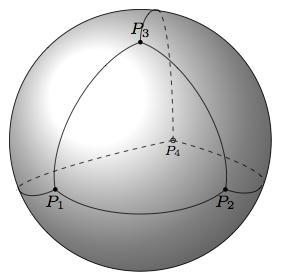
\includegraphics[height=5cm]{SphereTetrahedron}
    \caption{Triangulating a Sphere. (googled image)}
	\end{figure}
  \vspace{6em}
\end{addmargin}


\noindent \textbf{Question 5.} Good cover for $X \vee Y$:\\
\begin{addmargin}[2em]{0em}
In general, if $X$ and $Y$ have good covers $\U$ and $\U'$ such that the `point of gluing' belongs to a unique $U \in \U$ and $U' \in \U'$. Then we can just use the open covers $\U$ and $\U'$ but glue the open sets $U$ and $U'$ at a point. We can easily check that this indeed forms a good cover. The only non-trivial fact needed to be shown is that if $U$ and $U'$ are contractible then so is $U \vee U'$ (exercise).
\end{addmargin}


\newpage

\noindent \textbf{Question 2. b)} If $X \times Y$ is contractible then so is $X$:\\
\begin{addmargin}[2em]{0em}
(I think you don't need the contractibility of $Y$, if you find a flaw in the following proof please let me know.)

Because $X \times Y$ is contractible, there is a point $(x_0, y_0) \in X \times Y$ and a continuous map
\begin{align*}
  \Phi: X \times Y \times [0,1] \rightarrow X \times Y
\end{align*}
such that
\begin{align*}
  \Phi(x,y,0) & = (x,y)   \\
  \Phi(x,y,1) & = (x_0,y_0)
\end{align*}
for all $ (x,y) \in X \times Y$ i.e. there are ``continuously varying paths'' connecting each point in $ X \times Y$ to $ (x_0,y_0)$.

Restrict the map $\Phi$ to $X \times \{ y_0 \}$ so that we get a map
\begin{align*}
  \Phi|_{y=y_0}: X \times [0,1] &\rightarrow X \times Y \\
  (x,t) &\mapsto \Phi(x,y_0,t)
\end{align*}
This is almost the map we want. Now we compose with the projection onto the first component $\pi_X: X \times Y \rightarrow X$ to get a map $\Psi = \pi_X \circ \Phi$
\begin{align*}
  \Psi : X \times [0,1] \xrightarrow{\Phi|_{y=y_0}} X \times Y \xrightarrow{\pi_X} X
\end{align*}
One can check that $\Psi(x,0) = x $ and $\Psi(x,1) = x_0$. Further, $\Psi$ is continuous as it is a composition of two continuous functions and hence $\Psi$ witnesses the contractibility of $X$.

(Try to draw pictures of what this proof is saying geometrically.)
\end{addmargin}

\end{document}
